\documentclass{standalone}
\usepackage{tikz}
\usetikzlibrary{patterns, positioning}
\usepackage[sfdefault]{ClearSans} %% option 'sfdefault' activates Clear Sans as the default text font
\usepackage[T1]{fontenc}

\begin{document}
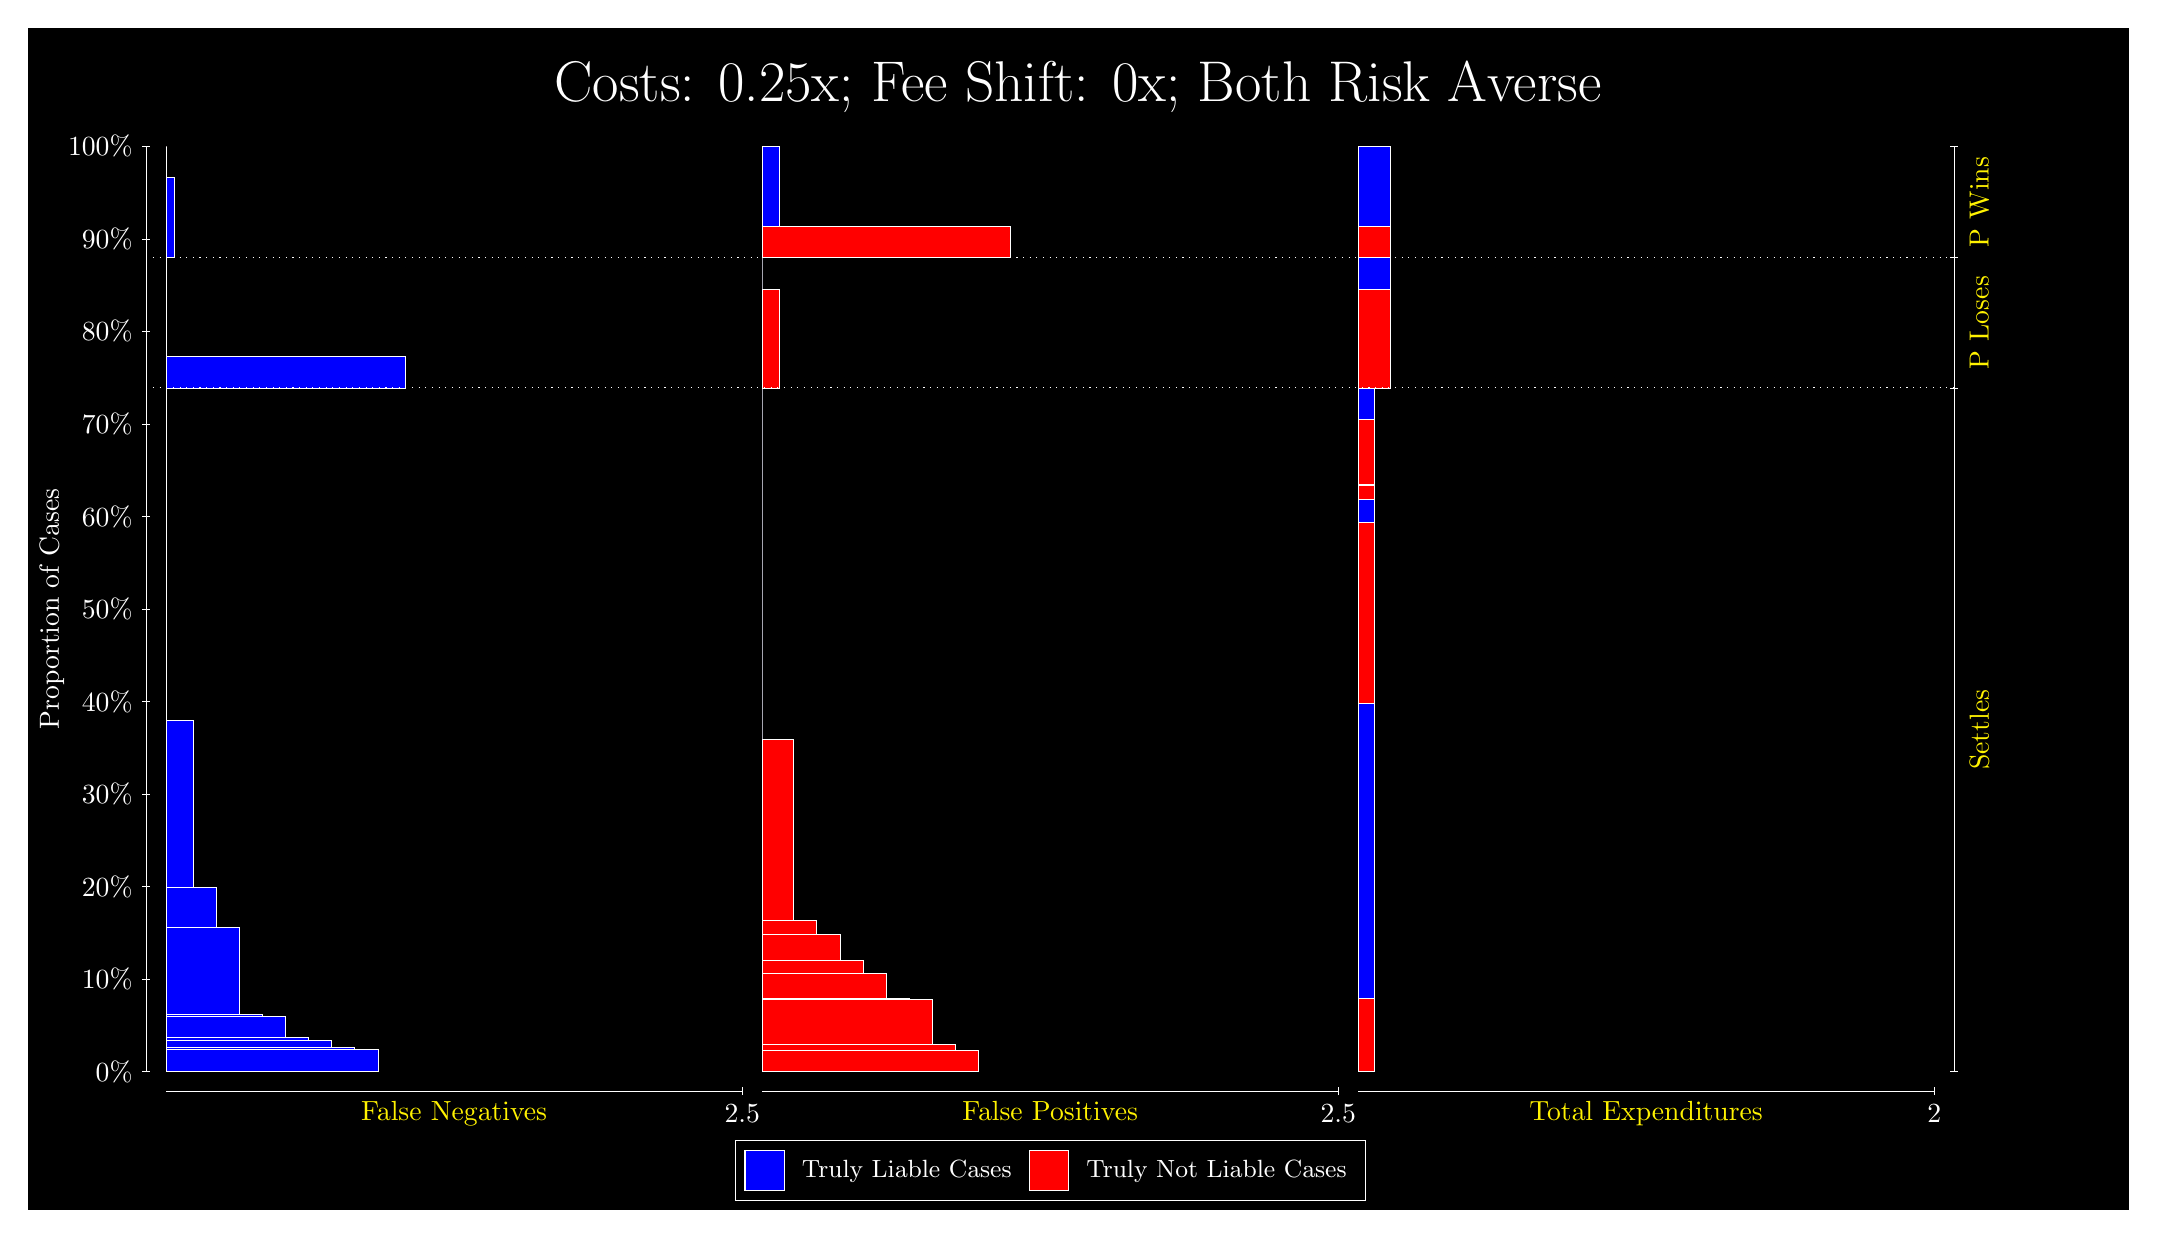
\begin{tikzpicture}
\draw[fill=black] (0,0) rectangle (26.667,15);
\draw[text=white] (0,13.5) rectangle (26.667,15) node[midway] {\huge Costs: 0.25x; Fee Shift: 0x; Both Risk Averse};
\draw[white, very thin] (1.5,1.75) -- (1.5,13.5);
\node[rotate=90, text=white, anchor=center] at (0.3, 7.625) {Proportion of Cases};
\draw[white, very thin] (1.45,1.75) -- (1.55,1.75);
\node[text=white, anchor=east] at (1.45, 1.75) {0\%};
\draw[white, very thin] (1.45,2.925) -- (1.55,2.925);
\node[text=white, anchor=east] at (1.45, 2.925) {10\%};
\draw[white, very thin] (1.45,4.1) -- (1.55,4.1);
\node[text=white, anchor=east] at (1.45, 4.1) {20\%};
\draw[white, very thin] (1.45,5.275) -- (1.55,5.275);
\node[text=white, anchor=east] at (1.45, 5.275) {30\%};
\draw[white, very thin] (1.45,6.45) -- (1.55,6.45);
\node[text=white, anchor=east] at (1.45, 6.45) {40\%};
\draw[white, very thin] (1.45,7.625) -- (1.55,7.625);
\node[text=white, anchor=east] at (1.45, 7.625) {50\%};
\draw[white, very thin] (1.45,8.8) -- (1.55,8.8);
\node[text=white, anchor=east] at (1.45, 8.8) {60\%};
\draw[white, very thin] (1.45,9.975) -- (1.55,9.975);
\node[text=white, anchor=east] at (1.45, 9.975) {70\%};
\draw[white, very thin] (1.45,11.15) -- (1.55,11.15);
\node[text=white, anchor=east] at (1.45, 11.15) {80\%};
\draw[white, very thin] (1.45,12.325) -- (1.55,12.325);
\node[text=white, anchor=east] at (1.45, 12.325) {90\%};
\draw[white, very thin] (1.45,13.5) -- (1.55,13.5);
\node[text=white, anchor=east] at (1.45, 13.5) {100\%};

\draw[white, very thin] (24.457,1.75) -- (24.457,13.5);
\draw[white, very thin] (24.407,1.75) -- (24.507,1.75);
\node[anchor=west] at (24.407, 1.75) {};
\draw[white, very thin] (24.407,10.433) -- (24.507,10.433);
\node[anchor=west] at (24.407, 10.433) {};
\draw[white, very thin] (24.407,12.086) -- (24.507,12.086);
\node[anchor=west] at (24.407, 12.086) {};
\draw[white, very thin] (24.407,13.5) -- (24.507,13.5);
\node[anchor=west] at (24.407, 13.5) {};

\draw[white, very thin, fill=blue] (1.75,1.75) rectangle (4.4397,2.0359);
\draw[white, very thin, fill=blue] (1.75,2.0359) rectangle (4.1469,2.055);
\draw[white, very thin, fill=blue] (1.75,2.055) rectangle (3.8542,2.1477);
\draw[white, very thin, fill=blue] (1.75,2.1477) rectangle (3.5614,2.1897);
\draw[white, very thin, fill=blue] (1.75,2.1897) rectangle (3.2687,2.4576);
\draw[white, very thin, fill=blue] (1.75,2.4576) rectangle (2.9759,2.4724);
\draw[white, very thin, fill=blue] (1.75,2.4724) rectangle (2.6832,3.5854);
\draw[white, very thin, fill=blue] (1.75,3.5854) rectangle (2.3904,4.0894);
\draw[white, very thin, fill=blue] (1.75,4.0894) rectangle (2.0976,6.2105);
\draw[white, very thin, fill=red] (1.75,6.2105) rectangle (1.75,10.433);
\draw[white, very thin, fill=blue] (1.75,10.433) rectangle (4.7873,10.832);
\draw[white, very thin, fill=red] (1.75,10.832) rectangle (1.75,12.086);
\draw[white, very thin, fill=blue] (1.75,12.086) rectangle (1.8598,13.102);
\draw[white, very thin, fill=red] (1.75,13.102) rectangle (1.75,13.5);
\draw[white, very thin, fill=red] (9.3189,1.75) rectangle (12.063,2.0168);
\draw[white, very thin, fill=red] (9.3189,2.0168) rectangle (11.771,2.0903);
\draw[white, very thin, fill=red] (9.3189,2.0903) rectangle (11.478,2.6735);
\draw[white, very thin, fill=red] (9.3189,2.6735) rectangle (11.185,2.6802);
\draw[white, very thin, fill=red] (9.3189,2.6802) rectangle (10.892,2.9994);
\draw[white, very thin, fill=red] (9.3189,2.9994) rectangle (10.6,3.1653);
\draw[white, very thin, fill=red] (9.3189,3.1653) rectangle (10.307,3.4984);
\draw[white, very thin, fill=red] (9.3189,3.4984) rectangle (10.014,3.675);
\draw[white, very thin, fill=red] (9.3189,3.675) rectangle (9.7214,5.9726);
\draw[white, very thin, fill=blue] (9.3189,5.9726) rectangle (9.3189,10.433);
\draw[white, very thin, fill=red] (9.3189,10.433) rectangle (9.5384,11.688);
\draw[white, very thin, fill=blue] (9.3189,11.688) rectangle (9.3189,12.086);
\draw[white, very thin, fill=red] (9.3189,12.086) rectangle (12.466,12.484);
\draw[white, very thin, fill=blue] (9.3189,12.484) rectangle (9.5384,13.5);
\draw[white, very thin, fill=red] (16.888,1.75) rectangle (17.094,2.6802);
\draw[white, very thin, fill=blue] (16.888,2.6802) rectangle (17.094,6.4331);
\draw[white, very thin, fill=red] (16.888,6.4331) rectangle (17.094,8.7308);
\draw[white, very thin, fill=blue] (16.888,8.7308) rectangle (17.094,9.0167);
\draw[white, very thin, fill=red] (16.888,9.0167) rectangle (17.094,9.1933);
\draw[white, very thin, fill=blue] (16.888,9.1933) rectangle (17.094,9.2124);
\draw[white, very thin, fill=red] (16.888,9.2124) rectangle (17.094,10.031);
\draw[white, very thin, fill=blue] (16.888,10.031) rectangle (17.094,10.433);
\draw[white, very thin, fill=red] (16.888,10.433) rectangle (17.299,11.688);
\draw[white, very thin, fill=blue] (16.888,11.688) rectangle (17.299,12.086);
\draw[white, very thin, fill=red] (16.888,12.086) rectangle (17.299,12.484);
\draw[white, very thin, fill=blue] (16.888,12.484) rectangle (17.299,13.5);
\draw[white, dotted] (1.5,10.433) -- (24.457,10.433);
\draw[white, dotted] (1.5,12.086) -- (24.457,12.086);
\draw[white, very thin] (1.75,1.5) -- (9.0689,1.5);
\node[text=yellow, anchor=north] at (5.4094, 1.5) {False Negatives};
\draw[white, very thin] (9.0689,1.45) -- (9.0689,1.55);
\node[text=white, anchor=north] at (9.0689, 1.45) {2.5};

\draw[white, very thin] (9.3189,1.5) -- (16.638,1.5);
\node[text=yellow, anchor=north] at (12.978, 1.5) {False Positives};
\draw[white, very thin] (16.638,1.45) -- (16.638,1.55);
\node[text=white, anchor=north] at (16.638, 1.45) {2.5};

\draw[white, very thin] (16.888,1.5) -- (24.207,1.5);
\node[text=yellow, anchor=north] at (20.547, 1.5) {Total Expenditures};
\draw[white, very thin] (24.207,1.45) -- (24.207,1.55);
\node[text=white, anchor=north] at (24.207, 1.45) {2};

\node[text=yellow, centered, rotate=90] at (24.777, 6.0916) {Settles};
\node[text=yellow, centered, rotate=90] at (24.777, 11.26) {P Loses};
\node[text=yellow, centered, rotate=90] at (24.777, 12.793) {P Wins};

\draw (12.978300999999998,1.5) node[draw=none] (baseCoordinate) {};
\begin{scope}[align=center]
        \matrix[scale=0.5, draw=white, below=0.5cm of baseCoordinate, nodes={draw}, column sep=0.1cm]{
            \node[rectangle, draw, minimum width=0.5cm, minimum height=0.5cm, fill=blue] {}; &
            \node[draw=none, font=\small, text=white] (B) {Truly Liable Cases}; &
            \node[rectangle, draw, minimum width=0.5cm, minimum height=0.5cm, fill=red] {}; &
            \node[draw=none, font=\small, text=white] (B) {Truly Not Liable Cases}; \\
            };
\end{scope}

\end{tikzpicture}
\end{document}